\chapter{DESAIN DAN IMPLEMENTASI}
\label{chap:desainimplementasi}

% Ubah bagian-bagian berikut dengan isi dari desain dan implementasi
Bab ini akan menjelaskan mengenai sistem perencanaan gerakan mobil otonom, mulai dari konfigurasi sensor pada Simulator mobil otonom, perancangan informasi dan parameter lingkungan berkendara pada Simulator mobil otonom, perancangan sistem berkendara mobil otonom, hingga perancangan arsitektur algoritma DQN yang digunakan dalam Tugas Akhir ini.


\section{Deskripsi Sistem}
\label{sec:deskripsisistem}

Sistem pada tugas akhir ini merupakan implementasi dari salah satu disiplin ilmu \textit{Deep Reinforcement Learning} yang berfungsi untuk menciptakan algoritma yang dapat melakukan manuver kendaraan otonom untuk bergerak melewati bundaran atau \textit{u-turn}. Blok diagram metodologi sistem yang digunakan pada penelitian ini dapat dilihat pada Gambar \ref{fig:blockdiagram}.

\section{Persiapan Lingkungan Simulasi}
\label{sec:simulasi}
Menggunakan simulator CARLA, digunakan map Town03 CARLA, yang memiliki bundaran dan u-turn untuk memfasilitasi pengerjaan tugas akhir. Digunakan bundaran berjumlah simpang empat seperti pada Gambar  \ref{fig:bundaran_town03}. Pada lingkungan ini, agent akan \textit{spawn }dari dua titik \textit{spawn} di sekitar bundaran.
\begin{figure}[H] 
	\centering
	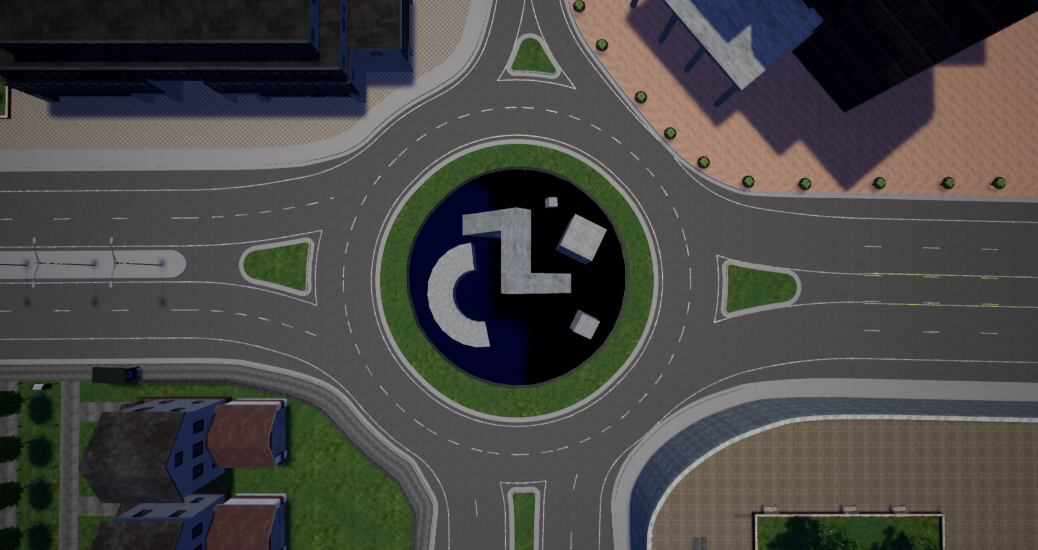
\includegraphics[width=.7\linewidth]{images/bundaran}
	\caption{Bundaran Town03}
	\label{fig:bundaran_town03}
\end{figure}

\section{Sensor}
\label{sec:sensor}
Sensor menggunakan sensor kamera yang diletakkan secara fisik di bagian depan bawah dari agen. Sensor kamera yang digunakan adalah sensor kamera segmentasi. Sensor kamera segmentasi adalah sensor kamera yang memisahkan object-object di simulator menjadi berbagai warna unik yang solid. Citra yang dihasilkan dari sensor kamera segmentasi pada Gambar \ref{fig:segmentasi} adalah citra lanjutan yang telah di proses dari citra RGB pada gambar \ref{fig:citra_rgb}


\section{Akuisisi Data}
\label{sec:akuisisi_data}
Data citra diambil dari sensor dengan ukuran 480x270. Citra yang digunakan adalah citra segmentasi yang telah disediakan oleh sensor kamera segmentasi dari CARLA Simulator.

\begin{figure}[H] 
	\centering
	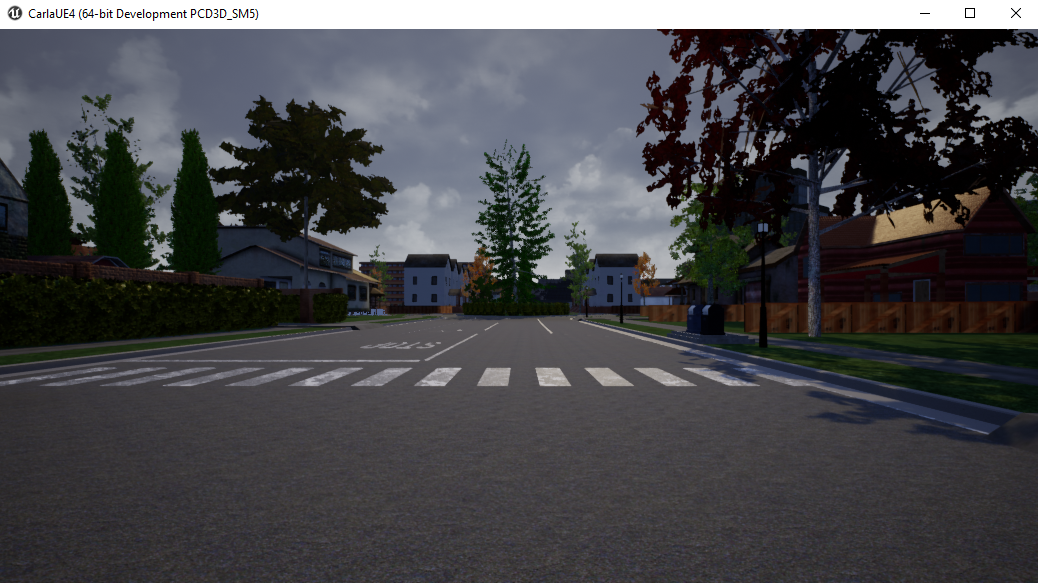
\includegraphics[width=.7\linewidth]{images/rgb}
	\caption{Citra RGB}
	\label{fig:citra_rgb}
\end{figure}
\begin{figure}[H] 
	\centering
	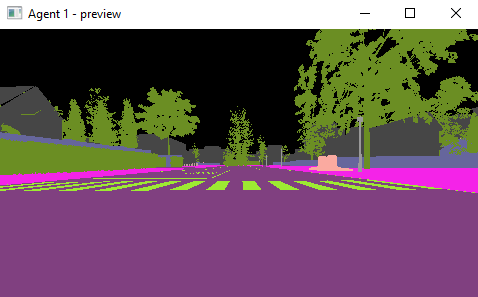
\includegraphics[width=.7\linewidth]{images/segmentasi}
	\caption{Citra Segmentasi}
	\label{fig:segmentasi}
\end{figure}
Citra segmentasi kemudian diberi filter grayscale agar dapat meminimalkan data yang dianalisa namun tetap mempertahankan fitur yang ada.
\begin{figure}[H] 
	\centering
	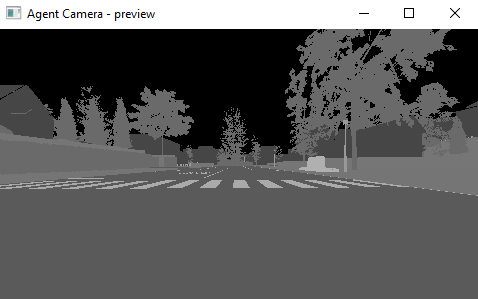
\includegraphics[width=.7\linewidth]{images/grayscale}
	\caption{Citra Grayscale}
	\label{fig:grayscale}
\end{figure}
Citra grayscale ini akan menjadi hasil akhir akuisi citra yang kemudian akan diberikan ke algoritma DQN untuk melakukan learning model dan/atau inference model.

\section{Action}
\label{sec:action}
Ada 3 action yang bisa dilakukan oleh agen. Diantaranya:

\begin{enumerate}[nolistsep]
	\item \verb=forward=
	
	Agent \textit{throttle} dengan nilai 1 dan \textit{steer} dengan nilai 0. Dengan demikian agent akan melakukan gerakan manuver maju.
	
	\item \verb=forward_left=
	
	Agen \textit{throttle} dengan nilai 1 dan \textit{steer} dengan nilai -1. Dengan demikian agent akan melakukan gerakan manuver maju ke depan kiri.

	\item \verb=forward_right=
	
	Agen \textit{throttle} dengan nilai 1 dan \textit{steer} dengan nilai 1. Dengan demikian agent akan melakukan gerakan manuver maju ke depan kanan.
	
\end{enumerate}

\section{Sistem Reward}
\label{sec:sistem_reward}

\subsection{Reward}
\label{sec:reward}
Fungsi reward dirancang agar mobil otonom mampu bergerak sepanjang lintasan dengan cepat dan aman. Ada dua buah reward yang ditetapkan dimana masing-masing reward memperhatikan referensi \textit{target lane}. Target lane adalah garis imajiner yang menjadi target gerakan mobil otonom. Terlihat pada Gambar \ref{fig:target_lane_line}, \textit{target lane} digambarkan dengan titik-titik merah di sekitar bundaran.

\begin{figure}[H] 
	\centering
	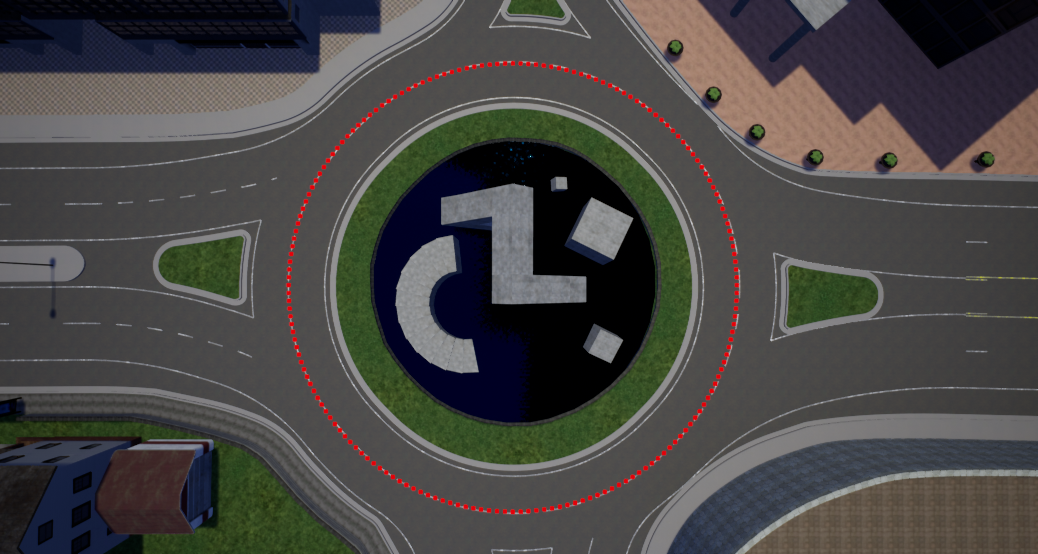
\includegraphics[width=1\linewidth]{images/target_lane_line}
	\caption{\textit{Target lane}}
	\label{fig:target_lane_line}
\end{figure}

\subsubsection{Reward 1: Deviasi sudut dari \textit{target lane}}
Reward yang digunakan pada Reward 1 adalah 1/alpha. Alpha adalah sudut agent yang menyimpang dari \textit{target lane}. Teknis alpha dijelaskan pada Gambar \ref{fig:reward_anglediff_sketch}. 

Garis hitam merupakan vektor tegak lurus antara titik pusat bundaran ke titik pusat agen. Lalu garis merah adalah vektor arah mobil. Dari kedua nilai tersebut, didapat alpha yang merupakan sudut dari kedua vektor tersebut. Kemudian nilai reward didefinisikan dengan 1/alpha.

\begin{figure}[H] 
	\centering
	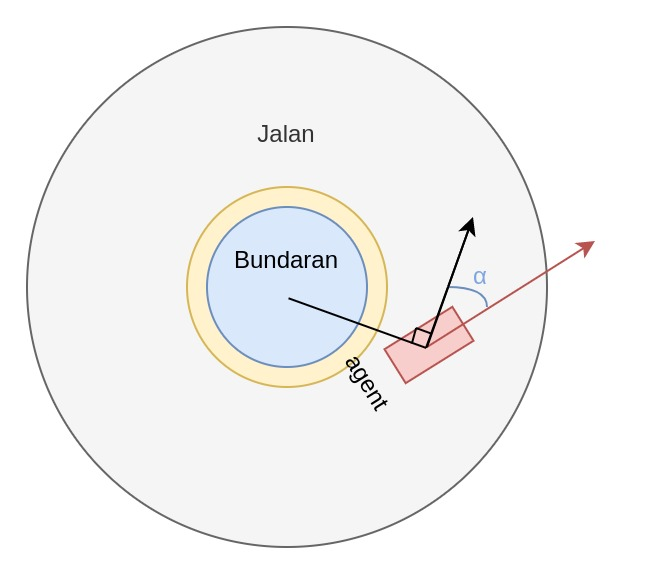
\includegraphics[width=1\linewidth]{images/reward_anglediff_sketch}
	\caption{Reward 1}
	\label{fig:reward_anglediff_sketch}
\end{figure}

\subsubsection{Reward 2: Deviasi jarak dari \textit{target lane}}
Reward yang digunakan pada reward 2 adalah \verb=1/deviasi_jarak*10=. Deviasi jarak adalah jarak terkecil agen terhadap \textit{target lane} dalam meter.

\subsection{Punishment}
\label{sec:punishment}
Punishment merupakan reward yang bernilai negatif. Ada dua punishment yang diberikan.

\subsubsection{Punishment 1: Sentuhan dengan obyek lain}
Reward senilai -1 akan diberikan pada \textit{agent} jika agent menyentuh object lain selain jalan raya, tanah, dan trotoar.

\subsubsection{Punishment 2: Deviasi jarak terlalu jauh}
Reward senilai -0.5 akan diberikan pada \textit{agent} jika jarak antara \textit{agent} dan bundaran lebih besar dari 30 meter. Jarak 30 meter dari bundaran dapat dilihat di Gambar \ref{fig:punishment_lane_line}

\begin{figure}[H] 
	\centering
	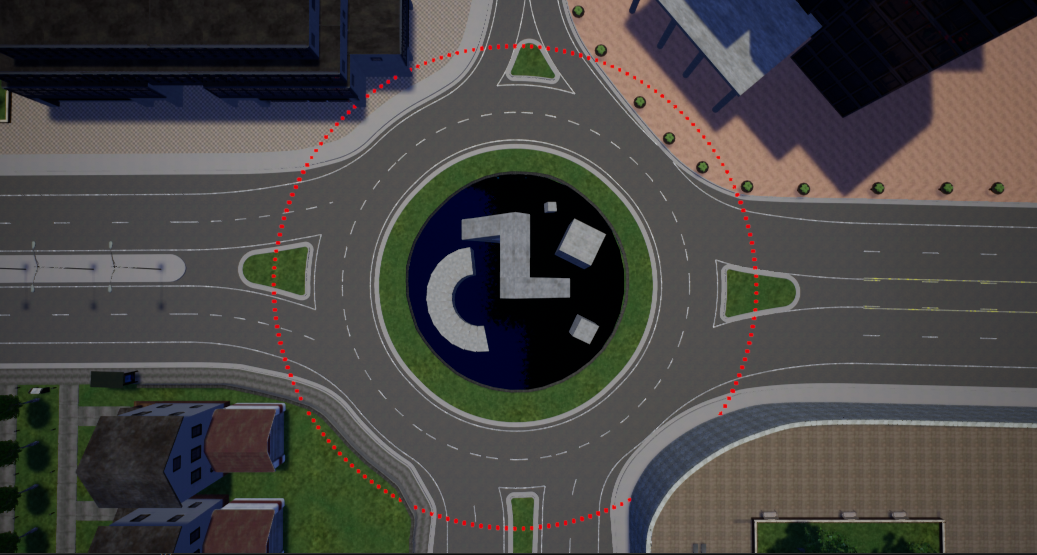
\includegraphics[width=1\linewidth]{images/punishment_lane_line}
	\caption{\textit{Punishment lane}}
	\label{fig:punishment_lane_line}
\end{figure}

\subsection{End Episode}
\label{sec:end_episode}
Waktu maksimal yang diberikan pada agent untuk melakukan proses learning setiap episodenya adalah 10 detik.

Episode akan berakhir jika waktu maksimal episode berakhir atau agent menyentuh object lain selain jalan raya, tanah, dan trotoar.

\section{Parameter DQN}
\label{sec:parameter_dqn}
Penentuan nilai hyperparameter yang tepat merupakan salah satu langkah yang penting dilakukan untuk mendapatkan model pembelajaran mesin yang baik. Dalam machine learning, hyperparameter adalah parameter yang digunakan untuk mengatur jalannya proses pembelajaran mesin. Berbeda dengan parameter model yang nilainya mengalami perubahan seiring berjalannya pembelajaran mesin, hyperparameter perlu didefinisikan di awal dan umumnya bernilai tetap sepanjang proses pembelajaran. Dalam tugas akhir ini, hyperparameter dari algoritma DQN didefinisikan sebagai berikut:

\subsection{Model}
\label{sec:model}
\begin{table}[H]
	\resizebox{\textwidth}{!}{%
		\begin{tabular}{|l|l|l|}
			\hline
			\textbf{Hyperparameter}   & \textbf{Nilai} & \textbf{Deskripsi}                                                                                                                            \\ \hline
			MINIBATCH\_SIZE           & 16             & \begin{tabular}[c]{@{}l@{}}Jumlah sampel pembelajaran yang\\ diproses oleh perhitungan SGD\\ (stochastic gradient) algoritma DQN\end{tabular} \\ \hline
			PREDICTION\_BATCH\_SIZE   & 1              & \begin{tabular}[c]{@{}l@{}}Jumlah sampel yang di prediksi\\ di saat yang bersamaan\end{tabular}                                               \\ \hline
			TRAINING\_BATCH\_SIZE     & 8              & \begin{tabular}[c]{@{}l@{}}Jumlah sampel yang di fit di saat\\ yang bersamaan (lebih besar lebih\\ cepat)\end{tabular}                        \\ \hline
			TRAINER\_MEMORY\_FRACTION & 0.6            &                                                                                                                                               \\ \hline
		\end{tabular}%
	}
\caption{Hyperparameter model.}
\label{tb:hyperparameter_model}
\end{table}

\iffalse
\begin{verbatim}
MINIBATCH_SIZE = 16
PREDICTION_BATCH_SIZE = 1
TRAINING_BATCH_SIZE = MINIBATCH_SIZE // 2
UPDATE_TARGET_EVERY = 100
TRAINER_MEMORY_FRACTION = 0.6
SAVE_CHECKPOINT_EVERY = 50
\end{verbatim}
\fi

\subsection{DQN}
\label{sec:dqn}

\begin{table}[H]
	\resizebox{\textwidth}{!}{%
		\begin{tabular}{|l|l|l|}
			\hline
			\textbf{Hyperparameter}   & \textbf{Nilai} & \textbf{Deskripsi}                                                                                                                            \\ \hline
			DISCOUNT                  & 0.99           & \begin{tabular}[c]{@{}l@{}}Nilai faktor discount dalam\\ perhitungan reward algoritma DQN\end{tabular}                                        \\ \hline
			REPLAY\_MEMORY\_SIZE      & 20\_000        & \begin{tabular}[c]{@{}l@{}}Berapa banyak step terakhir yang\\ disimpan untuk training model\end{tabular}                                      \\ \hline
			MIN\_REPLAY\_MEMORY\_SIZE & 5\_000         & \begin{tabular}[c]{@{}l@{}}Jumlah step minimum dalam\\ memori untuk memulai training\end{tabular}                                             \\ \hline
			OPTIMIZER\_LEARNING\_RATE & 0.001          & \begin{tabular}[c]{@{}l@{}}Laju pembelajaran yang digunakan\\ pada optimizer\end{tabular}                                                     \\ \hline
			OPTIMIZER\_DECAY          & 0.0            & \begin{tabular}[c]{@{}l@{}}Pengurangan laju pembelajaran\\ pada optimizer setiap episodenya\end{tabular}                                      \\ \hline
		\end{tabular}%
	}
	\caption{Hyperparameter DQN.}
	\label{tb:hyperparameter_dqn}
\end{table}

\iffalse
\begin{verbatim}
DISCOUNT = 0.99
REPLAY_MEMORY_SIZE = 20_000
MIN_REPLAY_MEMORY_SIZE = 5_000
\end{verbatim}
\fi

\subsection{Epsilon}

\begin{table}[H]
	\resizebox{\textwidth}{!}{%
		\begin{tabular}{|l|l|l|}
			\hline
			\textbf{Hyperparameter}   & \textbf{Nilai} & \textbf{Deskripsi}                                                                                                                            \\ \hline

			START\_EPSILON            & 1              & \begin{tabular}[c]{@{}l@{}}Nilai epsilon saat pertamakali\\ mulai training\end{tabular}                                                       \\ \hline
			EPSILON\_DECAY            & 0.9995         & \begin{tabular}[c]{@{}l@{}}Penurunan nilai epsilon di setiap\\ episodenya\end{tabular}                                                        \\ \hline
			MIN\_EPSILON              & 0.1            & \begin{tabular}[c]{@{}l@{}}Epsilon terendah yang\\ diperbolehkan\end{tabular}                                                                 \\ \hline
		\end{tabular}%
	}
	\caption{Hyperparameter epsilon.}
	\label{tb:hyperparameter_epsilon}
\end{table}
Penentuan parameter epsilon ditentukan oleh kondisi berikut. Epsilon akan bernilai 1 saat pertamakali memulai learning atau pada saat episode 0. Setiap dimulainya episode baru, nilai epsilon akan dikurangi sebanyak 0.9995 hingga pada akhirnya akan bernilai 0.1 setelah 1800 episode. Pengurangan nilai epsilon akan berhenti setelah sampai pada nilai 0.1.
\label{sec:epsilon}

\iffalse
\begin{verbatim}
START_EPSILON = 1
EPSILON_DECAY = 0.9995
MIN_EPSILON = 0.1
\end{verbatim}
\fi

\section{Arsitektur Model}
\label{sec:arsitektur_model}

Berikut adalah arsitektur yang digunakan:

\begin{table}[H]
	\begin{tabular}{lll}
		\textbf{Layer (type)}                      & \textbf{Output Shape}         & \textbf{Param \#} \\
		conv2d\_1\_input (InputLayer)     & (None, 270, 480, 1)  & 0        \\
		conv2d\_1 (Conv2D)                & (None, 270, 480, 64) & 640      \\
		activation\_1 (Activation)        & (None, 270, 480, 64) & 0        \\
		average\_pooling2d\_1 (AveragePoo & (None, 90, 160, 64)  & 0        \\
		conv2d\_2 (Conv2D)                & (None, 90, 160, 64)  & 36928    \\
		activation\_2 (Activation)        & (None, 90, 160, 64)  & 0        \\
		average\_pooling2d\_2 (AveragePoo & (None, 30, 54, 64)   & 0        \\
		conv2d\_3 (Conv2D)                & (None, 30, 54, 64)   & 36928    \\
		activation\_3 (Activation)        & (None, 30, 54, 64)   & 0        \\
		average\_pooling2d\_3 (AveragePoo & (None, 10, 18, 64)   & 0        \\
		flatten\_1 (Flatten)              & (None, 11520)        & 0        \\
		kmh\_input (InputLayer)           & (None, 1)            & 0        \\
		concatenate\_1 (Concatenate)      & (None, 11521)        & 0        \\
		dense\_1 (Dense)                  & (None, 256)          & 2949632  \\
		dense\_2 (Dense)                  & (None, 3)            & 771     
	\end{tabular}
\caption{Arsitektur model.}
\label{tb:arsitektur_model}
\end{table}

Diberikan konvolusi kepada citra image sebanyak 3 kali. Setiap konvolusi dilakukan dengan average pooling. Proses selanjutnya setelah konvolusi adalah menambahkan data kecepatan agent. Kemudian pada akhir dari proses akan didapatkan output action berjumlah 3.

Berikut adalah potongan program untuk model 64x3.
\lstinputlisting[
language=Python,
caption={Model 64x3.},
label={lst:bilanganprima}
]{program/model64x3.py}

Berikut adalah potongan program untuk hidden dense.
\lstinputlisting[
language=Python,
caption={Hidden dense.},
label={lst:bilanganprima}
]{program/hidden_dense.py}


\section{Training}
\label{sec:training}

\begin{figure}[H] 
	\centering
	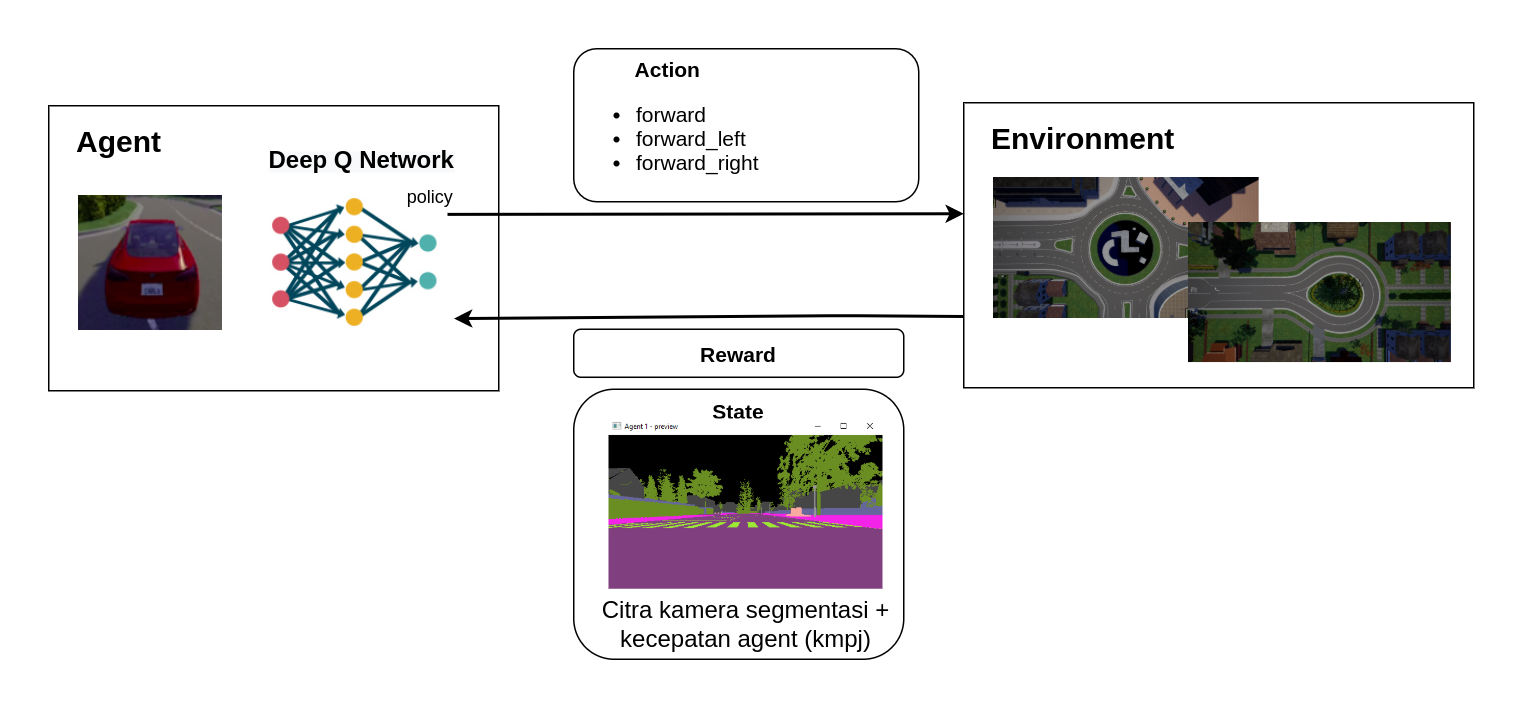
\includegraphics[width=1\linewidth]{images/metodologi}
	\caption{Diagram Blok Metodologi}
	\label{fig:blockdiagram}
\end{figure}
Tugas akhir ini akan menggunakan metode \textit{deep reinforcement learning}, yaitu \textit{reinforcement learning }yang disertai dengan \textit{deep learning }untuk mempelajari \textit{policy }apa yang cocok untuk digunakan oleh \textit{agent}. 

Algoritma deep reinforcement learning yang digunakan adalah Deep Q Network (DQN). Deep Q Network merupakan implementasi neural network atau deep learning pada Q-learning.

Parameter yang diberikan pada DQN adalah citra yang telah di segmentasi lalu diubah menjadi grayscale, serta kecepatan kendaraan dalam nilai kmpj.







%-----------------------------
%END for C and Python template
\iffalse
% Contoh pembuatan potongan kode
\begin{lstlisting}[
  language=C++,
  caption={Program halo dunia.},
  label={lst:halodunia}
]
#include <iostream>

int main() {
    std::cout << "Halo Dunia!";
    return 0;
}
\end{lstlisting}

% Contoh input potongan kode dari file
\lstinputlisting[
  language=Python,
  caption={Program perhitungan bilangan prima.},
  label={lst:bilanganprima}
]{program/bilangan-prima.py}

\lipsum[4]
\fi
